\sisetup{locale = EN} 
\begin{document}\selectlanguage{english}
\small
\section*{\huge{LHCb Quark-Puzzle}}
\begin{figure}[h]
    \begin{minipage}[t]{0.474\textwidth}
    %\vspace{-6.0cm}
        You have already learnt about the standard model of particle physics in the introductory lecture. In the illustration on the right, you can see the quarks.  Now it is your task to form particles from the smallest components of matter - the quarks. In the following, you will be given quarks and antiquarks that possess the knowledge of scientists in the construction of matter! What was nature thinking when it gave quarks these properties? Which particles can be built and under what conditions? 
    \end{minipage}~~
     \begin{minipage}[t]{0.50\textwidth}
     \centering
       \vspace{-1cm}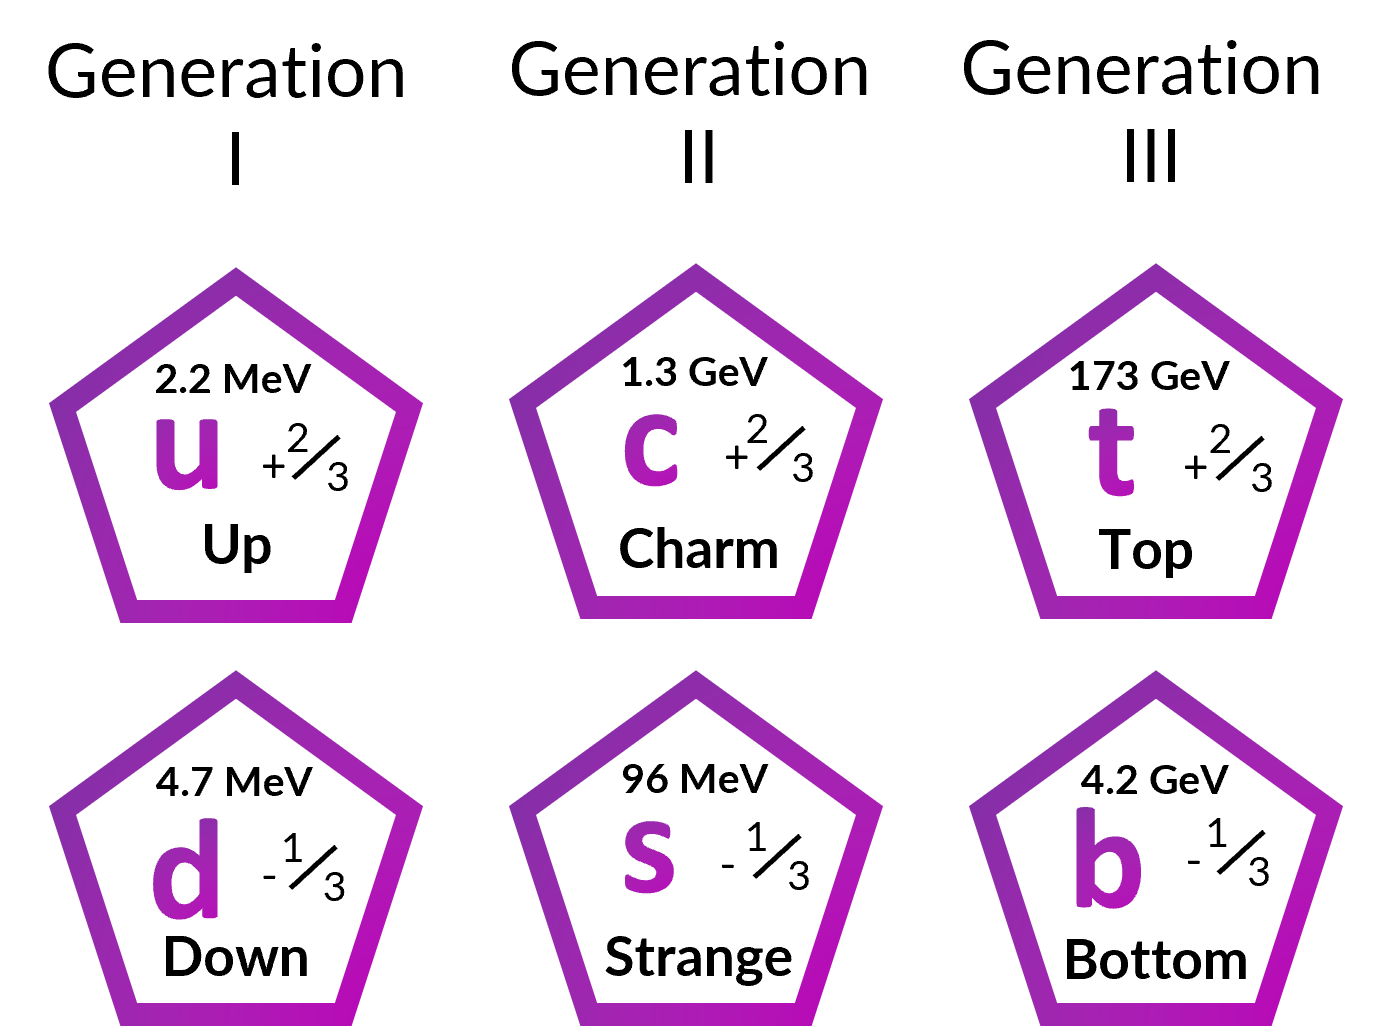
\includegraphics[width=.8\textwidth]{Figures Worksheets/Quarks_Quark_Puzzle_Worksheet.png}
         \caption{Overview of quarks, their masses and electric charges in units of $e$. The sign of the charge changes for antiquarks.}
    \end{minipage}
    \end{figure}
\SetDefinition{\textbf{On the trail of nature:} Build closed particles from quarks (e.g. u) and antiquarks (e.g. $\Bar{\textmd{u}}$). What are they called and under what conditions do quarks stick together to form a particle? Are there any peculiarities? \\ \emph{Work in groups and divide up the tasks:} \\ \, \\
\textbf{a)} Try it out! When you have found a particle, write down the letter combinations of the quarks (this is called the quark content) \\ \, \\ \textbf{b)}.
\textbf{b)} What are the names of your particles? Use your PC or smartphone to access the website \url{https://hadron-names.web.cern.ch} or use the QR code below! Enter the quark content in the bar. For antiquarks, use capital letters (U instead of $\Bar{\textmd{u}}$). Write names on the back!\\ \, \\
\textbf{c)} Look at your finished particles. What abnormalities, e.g. in the charge, colour, etc., can you discover? Make a note of these.
}

\emph{note}: \begin{enumerate*}[label=\textbf{\roman*)}]\item Please do not use force when putting the quarks together. If you can no longer separate a particle, please contact us. \item Holes can remain open. \item There is not \emph{the correct } solution. \item Can antiquarks bind with quarks?\end{enumerate*}
\\ \textcolor{white}{dummy} \hfill\, 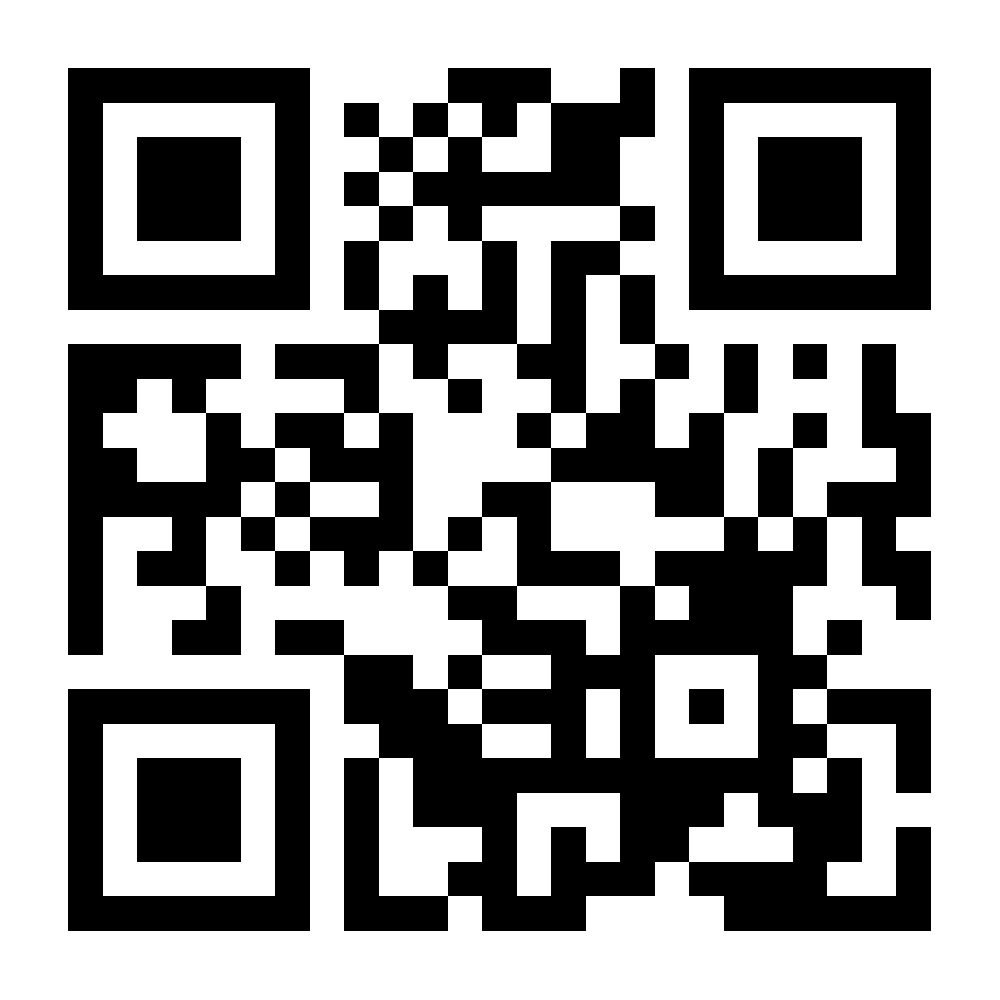
\includegraphics[width=2cm]{Figures Worksheets/qrcode.png}
\newpage
\checkered{Use this page for notes}{16}{23}


            
            
\end{document}